\documentclass[twocolumn,10pt]{article}
\usepackage[a4paper, top=0.65in, bottom=0.8in, left=0.65in, right=0.65in]{geometry}

\usepackage{graphicx}
\usepackage{algorithm}  
\usepackage{algorithmicx}  
\usepackage{algpseudocode}  
\usepackage{amsmath}
\usepackage{url}
\usepackage{xcolor}
\usepackage{listings}

\renewcommand{\algorithmicrequire}{\textbf{Input:}}  
\renewcommand{\algorithmicensure}{\textbf{Output:}}  
\graphicspath{{figure/}}

\lstdefinelanguage{swift}
{
	morekeywords={
		func,if,then,else,for,in,while,do,switch,case,default,where,break,continue,fallthrough,return,
		typealias,struct,class,enum,protocol,var,func,let,get,set,willSet,didSet,inout,init,deinit,extension,
		subscript,prefix,operator,infix,postfix,precedence,associativity,left,right,none,convenience,dynamic,
		final,lazy,mutating,nonmutating,optional,override,required,static,unowned,safe,weak,internal,
		private,public,is,as,self,unsafe,dynamicType,true,false,nil,Type,Protocol,
	},
	morecomment=[l]{//}, % l is for line comment
	morecomment=[s]{/*}{*/}, % s is for start and end delimiter
	morestring=[b]" % defines that strings are enclosed in double quotes
}
\definecolor{keyword}{HTML}{BA2CA3}
\definecolor{string}{HTML}{D12F1B}
\definecolor{comment}{HTML}{008400}
\lstset{
	language=swift,
	basicstyle=\ttfamily,
	showstringspaces=false, % lets spaces in strings appear as real spaces
	columns=fixed,
	keepspaces=true,
	keywordstyle=\color{keyword},
	stringstyle=\color{string},
	commentstyle=\color{comment},
}

\begin{document}

\date{July 11th, 2017}

\title{\bf Grouper: a Framework for Developing Mobile Applications using Secret Sharing and Untrusted Servers}

\author{
	Meng Li, 201620728  
	\\ Supervisor: Yasushi Shinjo
}

\maketitle

\section{Introduction}

Conventional mobile applications are built based on a client-server mode and require the central servers for storing shared data. 
The users of such mobile applications must fully trust the central servers. 
If central servers are compromised by hackers, user information may be revealed because data is often stored on the server in cleartext. 
Users may lose their data when service providers shut down their servers. 

To address these problems, we are developing Grouper, a framework for developing mobile applications. 
Grouper uses multiple untrusted servers for data transfer.
Data is divided into several pieces by a secret sharing scheme and uploaded to those untrusted servers. 
Each server can only keep a piece of data called a share. A share will be deleted after a period of time. 
These ensure that user data cannot be cracked easily. 
In addition, all devices of group members keep a complete data set of this group, and data can be recovered even untrusted servers shut down.

\section{Design of Grouper}

\subsection{Overview}

We are aiming at developing applications which are not relying on trusted central servers. 
The Grouper framework provides the following functions to applications.

\begin{itemize}
	\setlength{\itemsep}{1pt}
	\setlength{\parskip}{0pt}
	\setlength{\parsep}{0pt}
	\item Data Synchronization: If an user updates an object in his device, the mirrors of this object in other devices are updated.
	\item Group management: A group owner can create a group and invite other members to his group.
\end{itemize}

We implement data synchronization using the Sync framework\cite{sync} and our own messaging function called \emph{Grouper Message} Protocol.
Using the Sync framework, we get a JSON string from an updated object, send the JSON to other devices, and update the mirrors of the object in these devices. 
We implement \emph{Grouper Message} using untrusted servers and a secret sharing scheme  (Section 2.3). 
Untrusted servers delete messages after a period of time. 
\emph{Grouper Message} implements reliable messaging over this feature (Section 2.3).

\subsection{Threat Model}

We design Grouper based on data synchronization through multiple untrusted servers. Our untrusted servers have the following features.

Firstly, servers must perform device authentication. 
Servers generate access keys for group users. 
When a device wants to get/put data from/to untrusted servers, the device sends a request with an access key in the request header.

Secondly, servers keep data temporarily.
We define a period of time in which data can be kept in a server as an interval time. 
The data in untrusted servers vanishes after the interval time.

In members inviting, a group owner authenticates group members by a face-to-face way. We assume that inter-mobile device communication during this invitation time is secure. All group members must trust this group owner and they are not malicious.

\subsection{Data Synchronization}

\subsubsection{Data Transportation}

Figure 1 describes our data transportation flow using multiple untrusted servers. 
At first, the sender adds a record and Grouper creates three shares by a secret sharing scheme. 
In a secret sharing scheme, a member securely shares a secret with a group of members by generating $n$ shares using a cryptographic function. 
At least $k$ or more shares can reconstruct the secret, but $k-1$ or fewer shares can obtain nothing about the secret\cite{pang2005new}. 
We describe this scheme as a function $f(k, n)$, where $n$ is the number of all shares, and $k$ is the threshold to combine shares. 
 
Next, Grouper uploads those shares to three untrusted servers. 
In Figure 2, the receiver is online, and he downloads two shares from two servers and recovers the new record. 
In this process, these servers cannot recover user data because they do not have permission to access other untrusted servers. 

\begin{figure}[t]
	\centering
	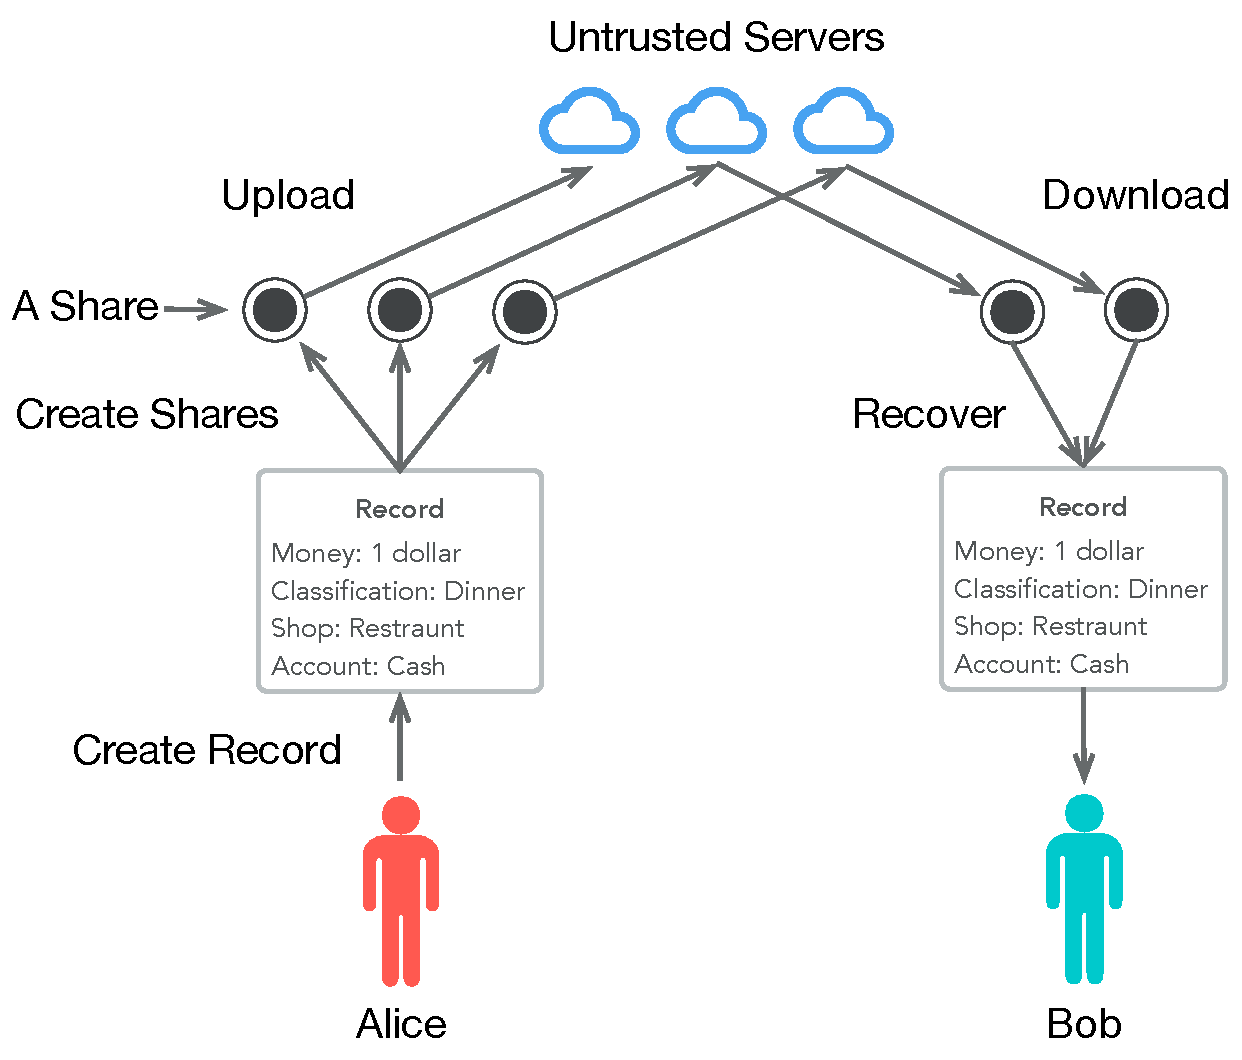
\includegraphics[scale=0.36]{sync_flow}
	\caption{Data transportation flow in Grouper.}
\end{figure}

\subsubsection{Reliable Synchronization}

Grouper should provide a reliable synchronization service. 
A user in a group creates a new record and all of other members in this group should synchronize this record, even if this record is deleted by untrusted servers after an interval time. 
We call this problem reliable synchronization. 
A receiver can only download shares from untrusted server with the interval time. 
If he is offline within the interval time, he will miss the new record.

\begin{figure}[t]
	\centering
	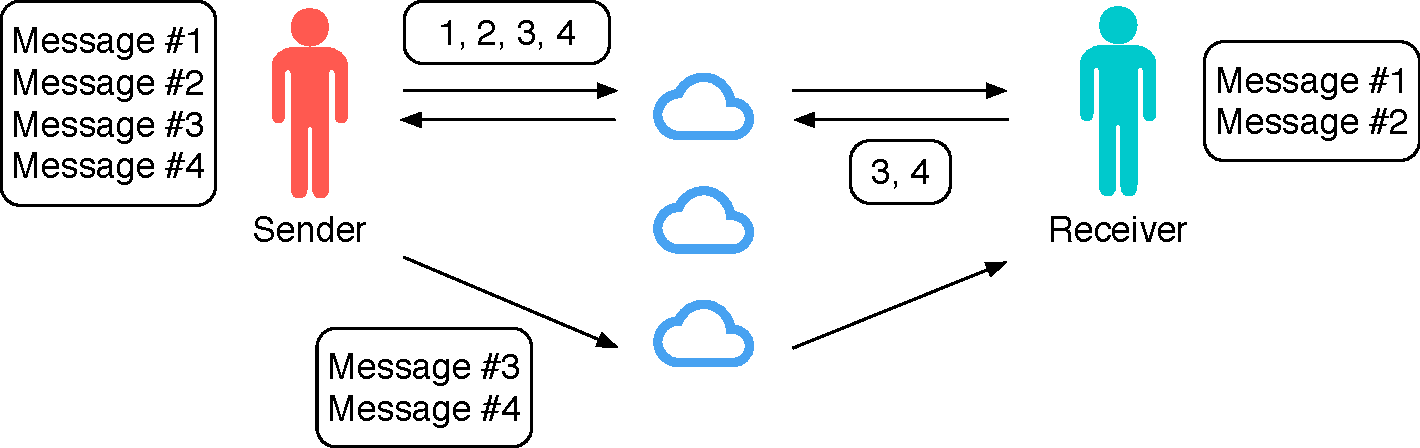
\includegraphics[scale=0.32]{reliable_sync}
	\caption{Reliable synchronization.}
\end{figure}

To solve this problem, we use the idea of reliable multicasting in distribute systems. 
In Figure 2, the sender has sent messages from No.1 to No.4. 
Next, he sends sequence numbers of all messages he sent to the receiver. 
When the receiver receives the sequence numbers, he checks his local persistent store. 
In this situation, the receiver finds that he missed the message No.3 and No.4. 
Thus, he will send a resend request that contains the sequence numbers of messages he missed to the sender. 
At last, the sender will send the message No.3 and No.4 again to the receiver again.

\subsubsection{Grouper Message Protocol}

To transfer data between devices, we design our own protocol, \emph{Grouper Message} Protocol. 
In this protocol, a message is a JSON string that contains an object of an application and the way to handle it in receivers’ devices. 
There are 4 types of Grouper messages: update message, delete message, confirm message and resend message. 
Both update message and delete message need resending because they contain the objects of an application. 
We call these messages normal messages. 
Both confirm message and resend message contain control information about reliable multicast and need not resending. 
We call these messages control messages.

When a user creates a new object or modifies some attributes of an existing object, the device sends an update message that contains the JSON string of this object to all group members.

When a user deletes an existing object, the device sends a delete message that contains the object ID of this object to all group members.

To confirm all devices have received all normal messages (update message and delete message) created by a user, the device sends a confirm message to all devices periodically. 
In this confirm message, the sequence number of objects recently created in this device are included.

When the device of a group member receives a confirm message, it checks the sequence numbers. 
If some of them do not exist in the persistent store, the device sends a resend message that contains missing sequence numbers.

\subsection{Group Management}

\subsubsection{Creating a Group}

A user creates a group, and he becomes the owner of this group.  
Before creating a group, the owner prepares his own user information including his email and name, multiple untrusted servers, a group ID and a group name. 
Next, he initializes this group on all untrusted server by submitting his node identifier. 
The node identifier, which represents his device, is generated by Grouper randomly when the application is launched at the first time. 
In each untrusted server, the Web service initializes this new group and returns a master key including the highest privilege to the owner. 
The owner can add other members to an untrusted server by the master key.

\subsubsection{Inviting a Member}

After creating a group, the owner can invite a new member to his group. 
To join the group, the new member prepares his user information at first. 
The owner invites the new member by a face-to-face way rather than using central servers. 
Before inviting, Grouper establishes connection between their devices using local secure links like \emph{Multipeer Connectivity}\cite{mc}. 
Firstly, the new member sends user information and a node identifier to the owner. 
Owner saves the user information and the node identifier of the new member to his device. 
Secondly, the owner registers the new member on multiple untrusted servers by submitting the node identifier of the new member. 
Thirdly, untrusted servers returns access keys for the new member to the owner. 
Lastly, the owner sends the access keys, server addresses and the list of existing members to the new member. 
After receiving them, the new member can access these untrusted servers with the keys.

\section{Implementation}

Grouper consists of a Web service (Section 3.1) running on multiple untrusted servers and a client framework (Section 3.2) for developing applications.

\subsection{Web Service}

Grouper needs its own Web service rather than using commercial general cloud services like Amazon S3, Google Cloud for the following reasons:

\begin{itemize}
	\setlength{\itemsep}{1pt}
	\setlength{\parskip}{0pt}
	\setlength{\parsep}{0pt}
	\item The Web service must provide reliable synchronization based on the \emph{Grouper Message} protocol.
	\item The Web service must ensure that shares are deleted after a prescriptive time.
\end{itemize}

Our Web service provides RESTful API to transfer data with clients. 
It runs on the Tomcat server that is an open source implementation of the Java Servlet, JavaServer Pages, Java Expression Language and Java WebSocket technologies. 
We use the Spring MVC, a  Web model-view-controller framework, to create our RESTful API, and Hibernate, an open source Java Object-Relational Mapping (ORM) framework, to save and operate objects in the Web service. 

Our Web service includes three kinds of entities. 
They are \emph{Group}, \emph{User} and \emph{Transfer} entities. 
A \emph{Group} entity saves a group ID, a group name and its owner. 
A \emph{User} entity saves the node identifier of a user, the access key for this user, and the group entity of this user. 
A \emph{Transfer} entity saves a share generated with a secret sharing scheme, the time when the user uploads the share. 
For each user, there is a unique access key for him in an untrusted server. For a group, one of a user is its owner who has the highest privilege of this group.

\subsection{Client}

Grouper's client framework is developed in Objective-C, and it supports developing applications on iOS, macOS, watchOS and tvOS . 
Figure 3 describes the architecture of client framework. It is based on the following frameworks.   

\begin{figure}[t]
	\centering
	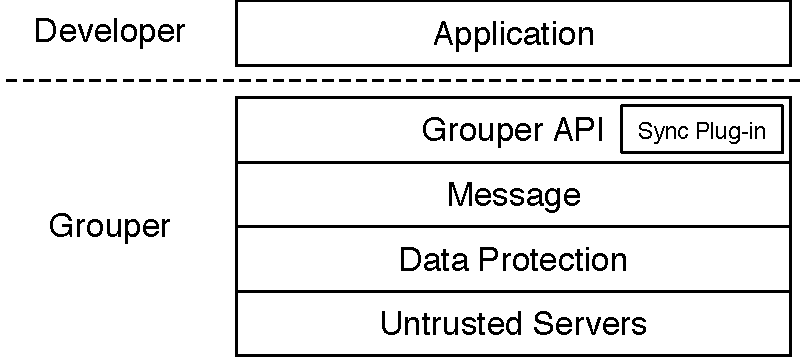
\includegraphics[scale=0.36]{architecture}
	\caption{Architecture of client.}
\end{figure}

\begin{itemize}
	\setlength{\itemsep}{1pt}
	\setlength{\parskip}{0pt}
	\setlength{\parsep}{0pt}
	\item 
	\emph{Multipeer Connectivity}\cite{mc},  an official Peer-to-Peer communication framework provided by Apple. 
	Grouper uses it to transfer data between two devices by a face-to-face way.
	\item 
	\emph{Core Data}\cite{coredata}, an official ORM framework provided by Apple.
	\emph{Core Data} provides generalized and automated solutions to common tasks associated with object life cycles and object graph management, including persistence. 
	Grouper uses it to manage model layer objects. 
	\item 
	\emph{Sync}\cite{sync}, a synchronization framework for \emph{Core Data} using JSON. 
	When a user sends messages, Grouper uses it to create JSON strings from objects. 
	When an other user receives messages, Grouper uses it to parse JSON strings and synchronize the recovered objects into \emph{Core Data}.
	\item 
	\emph{c-SSS}\cite{c-sss}, an implementation of the secret sharing scheme.
	\item 
	\emph{AFNetworking}\cite{afnetworking}, a delightful networking library in Objective-C. 
	Grouper uses it to invoke the RESTful API provided by our Web services running on multiple untrusted servers. 
\end{itemize}

\subsection{Applications}

Using Grouper framework, we are developing the following applications. 

\begin{itemize}
	\setlength{\itemsep}{1pt}
	\setlength{\parskip}{0pt}
	\setlength{\parsep}{0pt}
	\item \emph{Account Book}, an iOS application in Objective-C, records the income and expenditure of a group.
	\item \emph{Test}, a benchmark iOS aapplication in Swift, tests the performance of Grouper.
	\item \emph{Notes}, a macOS application in Swift, takes shared notes for a small group.
\end{itemize}

\section{Evaluation}

This section shows the developer efforts to use Grouper and the performance of Grouper.

\subsection{Developer Efforts}

We see developer efforts through two factors: the usability of the client API and the code size in the lines of code(LoC) the developer has to add after using Grouper. 
Grouper provides the following simple client API for developers.

\begin{lstlisting}
// Setup Grouper with appId and dataStack.
grouper.setup(withAppId:"id",
  dataStack:DataStack(modelName: "name"))
// Update an object.
grouper.sender.update(object)
// Delete an object.
grouper.sender.delete(object)
// Receive objects.
grouper.receiver.receive { 
  // Callback after receiving objects.
}
// Send a confirm message.
grouper.sender.confirm()
\end{lstlisting}

We have developed two applications including \emph{Account Book} and \emph{Test} with Grouper. 
As described in Table 1, based on the stand alone application without data synchronization, developers can add data synchronization to these applications with Grouper by adding a small number of code. 

\begin{table}[!htb]
	\footnotesize
	\centering  
	\caption{Applications' lines of code}
	\begin{tabular}{c|c|c}
		\hline
		Application Name           & Test  & Account Book \\ \hline
		Platform            & iOS   & iOS          \\ \hline
		Lanaguage           & Swift & Objective-C  \\ \hline
		Number of Entities  & \multicolumn{1}{r|}{1}     & \multicolumn{1}{r}{5}            \\ \hline
		Stand Alone Application LoC     & \multicolumn{1}{r|}{621}   & \multicolumn{1}{r}{8760}         \\ \hline
		Application with Groper LoC     &  \multicolumn{1}{r|}{632}   & \multicolumn{1}{r}{8950}         \\ \hline
		Increased LoC & \multicolumn{1}{r|}{11}    & \multicolumn{1}{r}{190}           \\ \hline
	\end{tabular}
\end{table}

\subsection{Performance}

The performance goal is to avoid significantly affecting the user experience with the application developed with Grouper. 
To evaluate whether Grouper meets this goal, we use the benchmark application \emph{Test} with the $f(2, 3)$ secret sharing scheme to transfer data between iPhone 4s and iPod 5 generation on a wireless LAN network (802.11n). 
Both iPhone 4s and iPod 5 generation have A5 CPU and 512MB of RAM.

\begin{figure}[t]
	\centering
	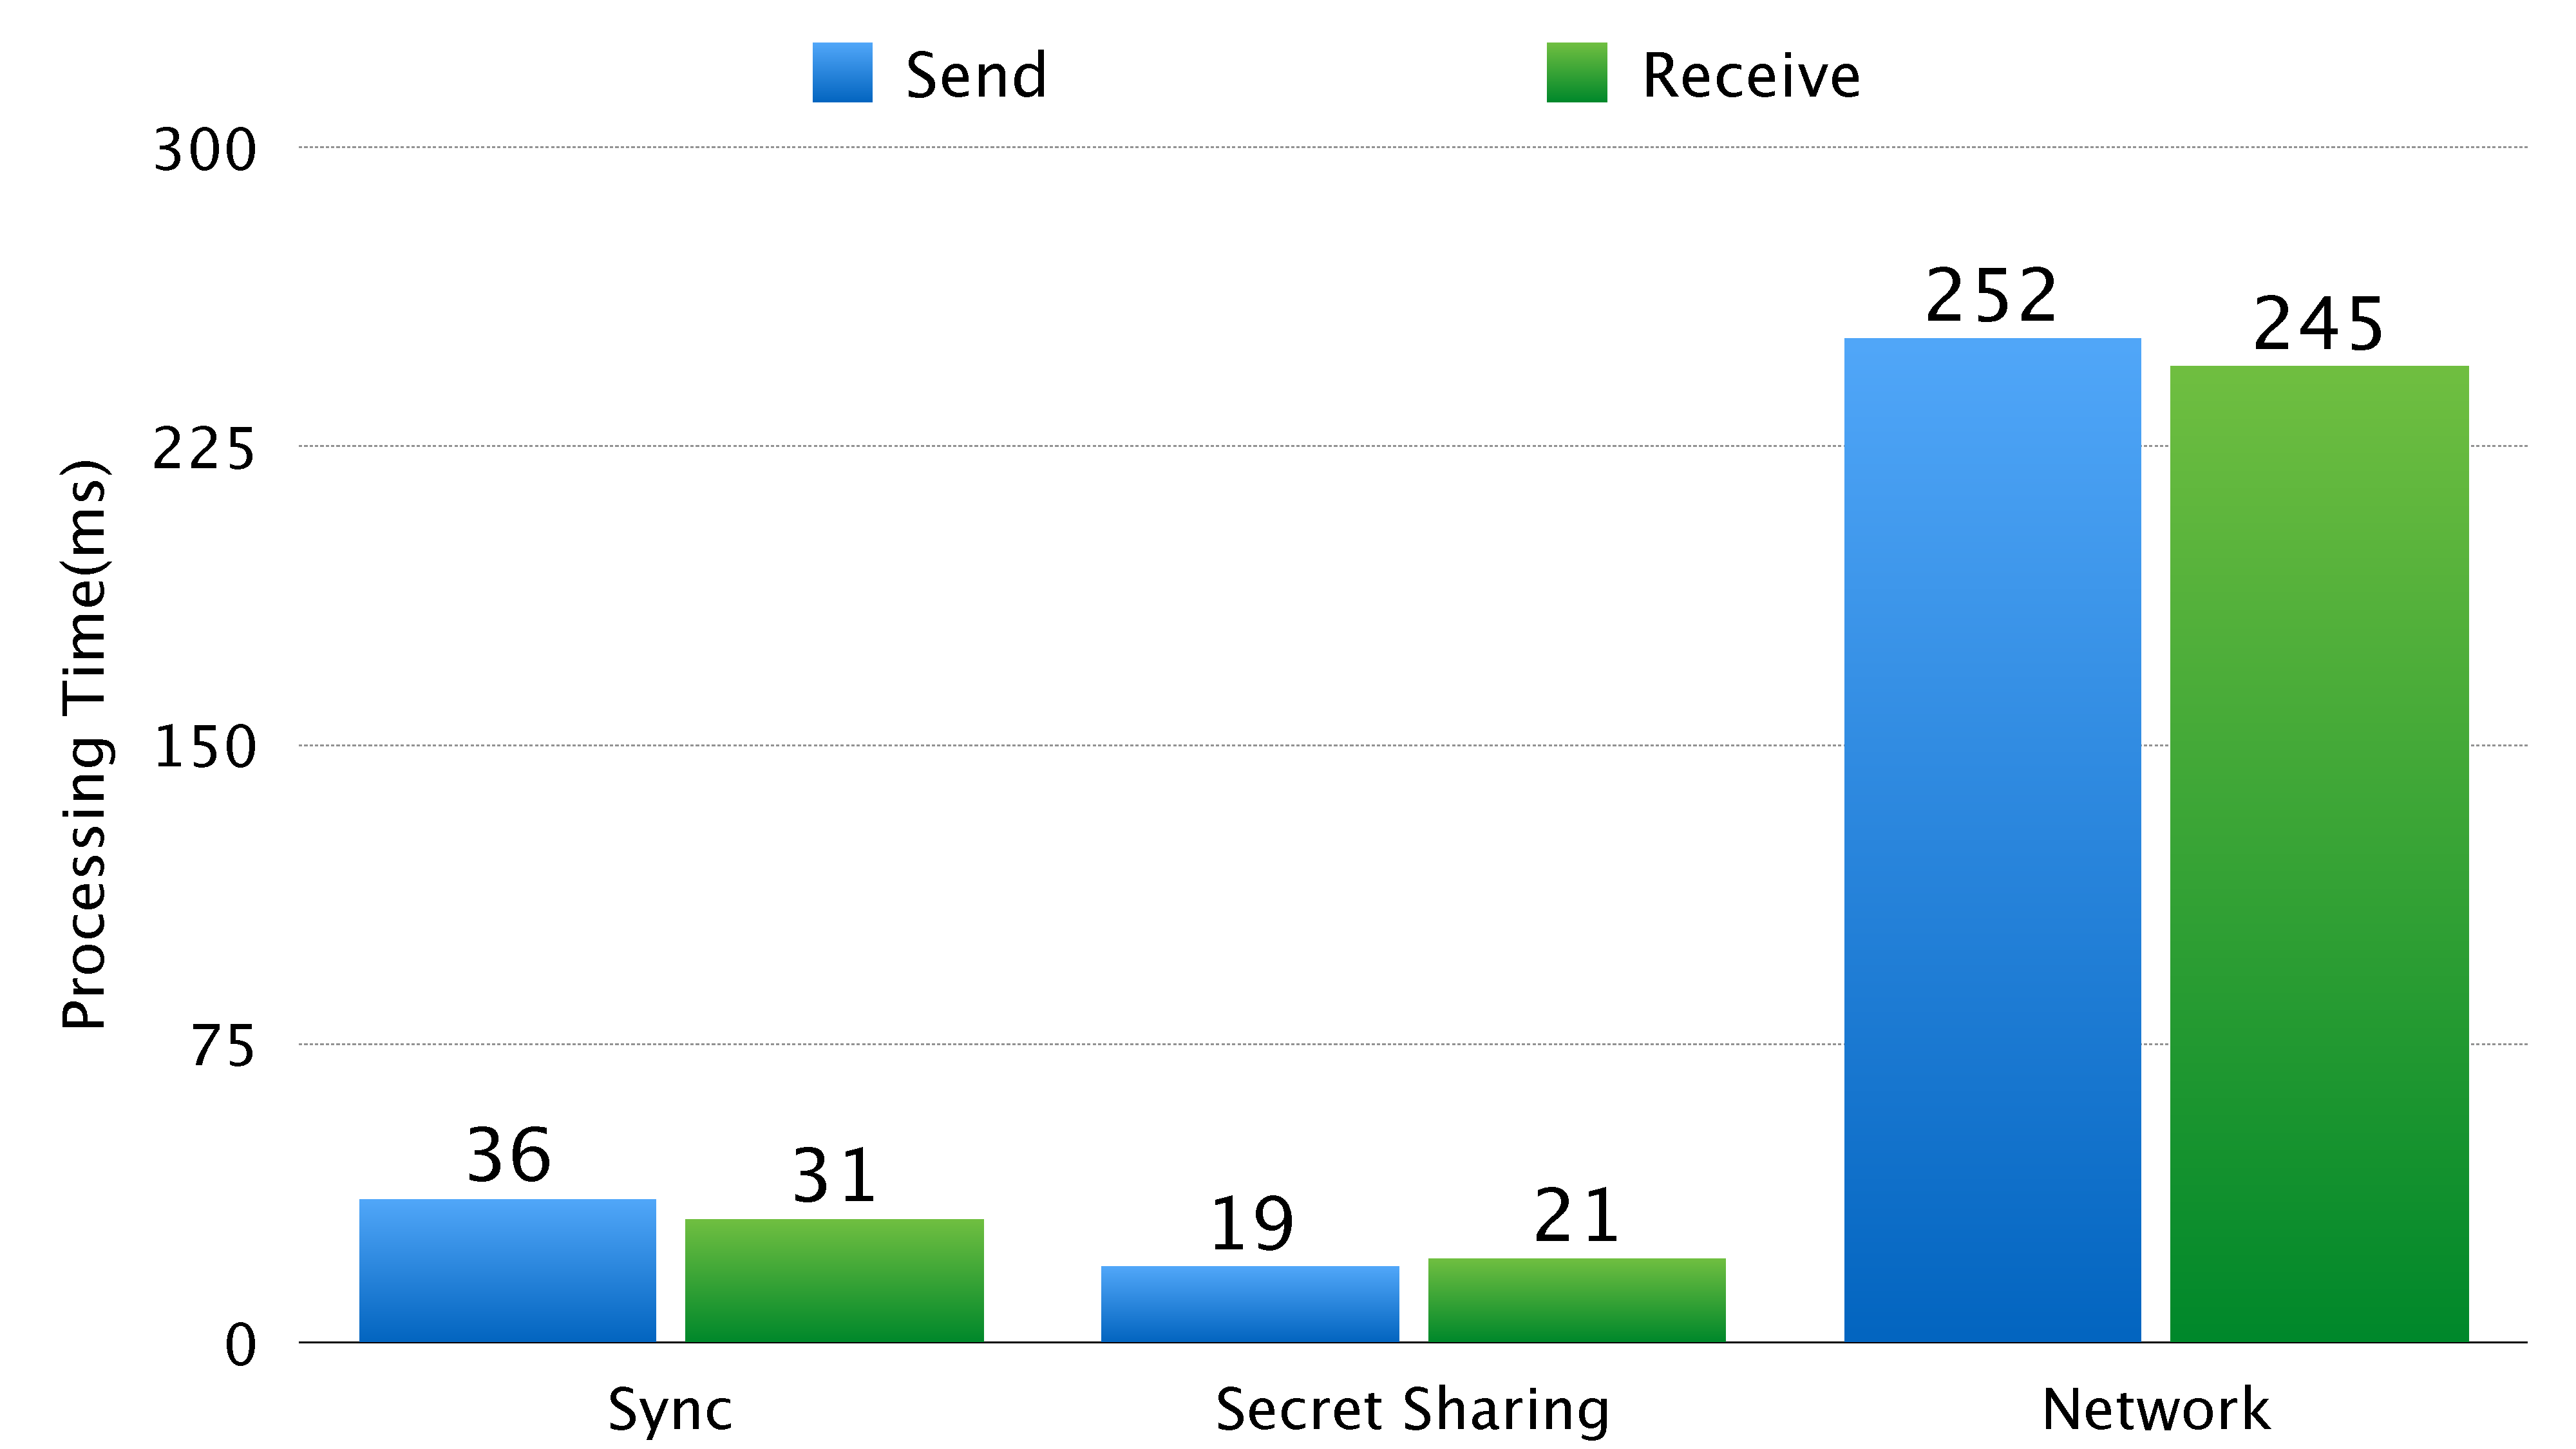
\includegraphics[scale=0.12]{processing1}
	\caption{Sending and receiving a single message.}
\end{figure}

\begin{figure}[t]
	\centering
	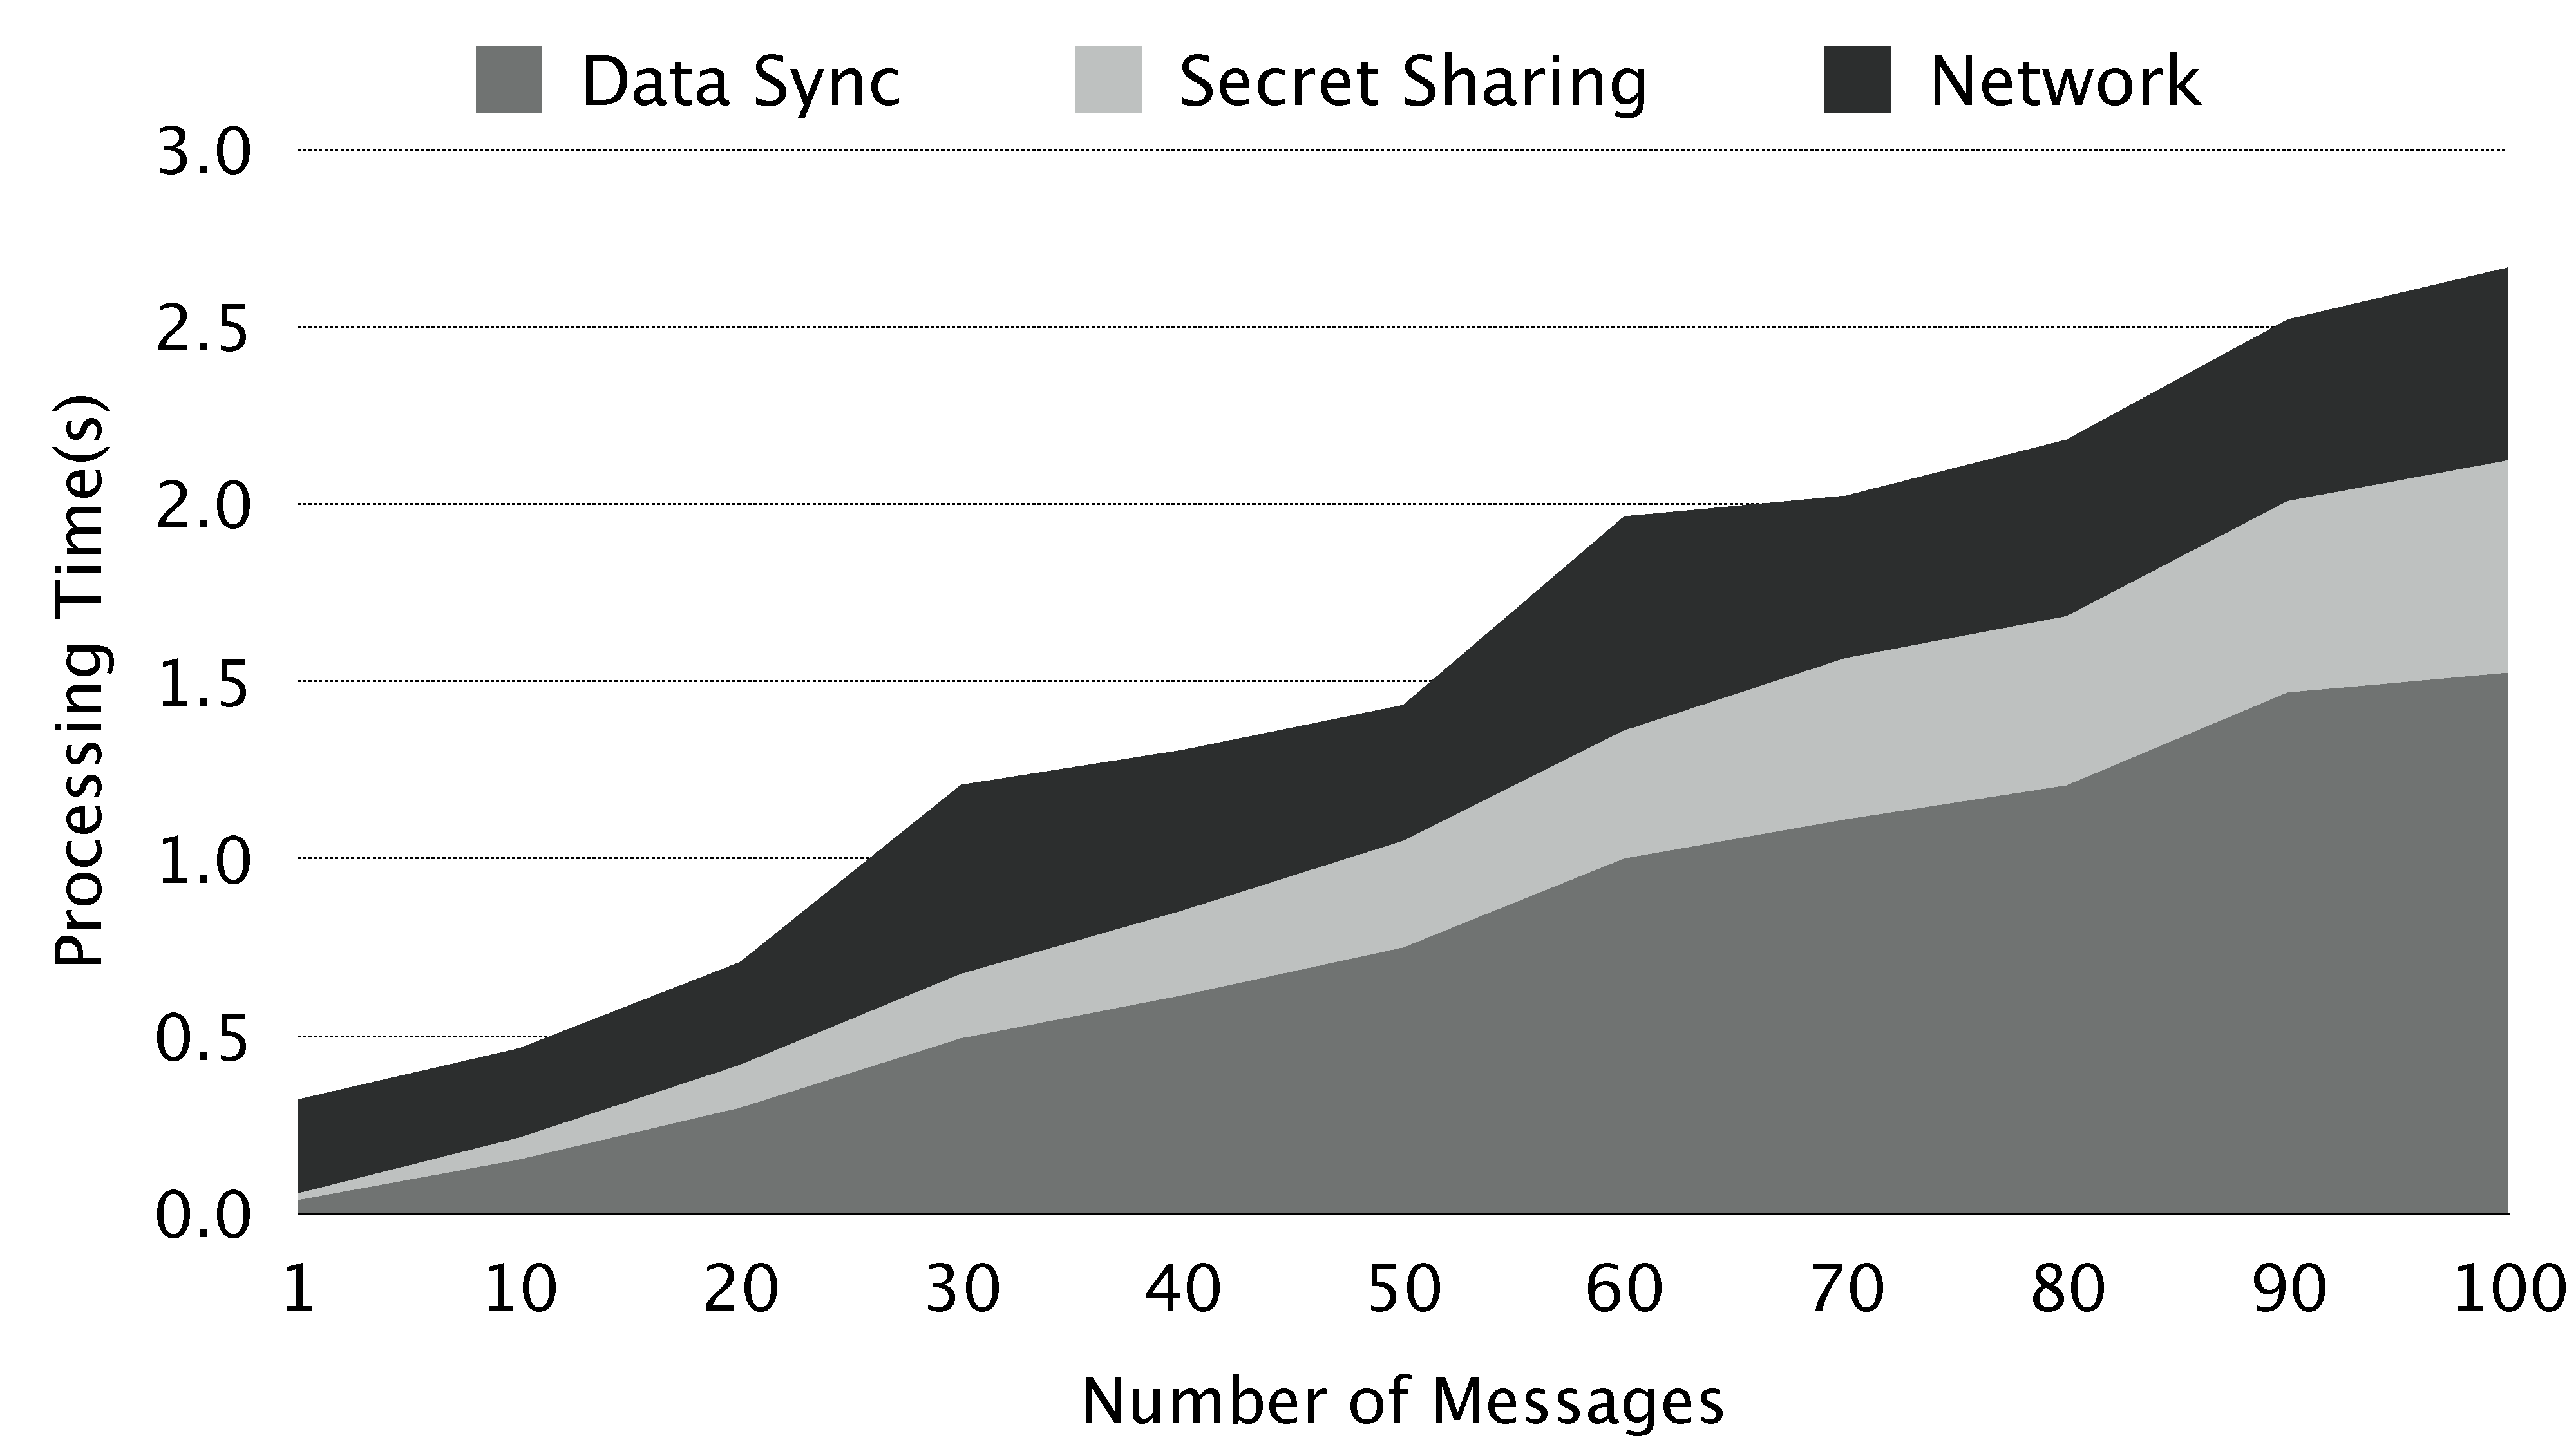
\includegraphics[scale=0.12]{processing2}
	\caption{Sending multiple messages.}
\end{figure}

First, we measured processing times the benchmark application \emph{Test} needed when a user created a test object during online. 
We used iPhone 4s to create an object and send a update message. 
We used iPod 5 generation to receive the update message from iPhone 4s.
Figure 4 shows the processing time for sending and receiving a single message after creating this object.
This size of the message was 620 bytes.
Compared to the network time, data sync and secret sharing consumed very little time in both data sending and receiving.

Next, we measured processing times \emph{Test} needed when a device sent update messages to untrusted servers.
We used iPod 4s to create multiple objects and to send multiple update messages at the same time.
Figure 5 shows the processing time for sending multiple messages. 
As the number of messages increased, data sync and secret sharing part increased linearly. 
The network part increased very slowly and sometimes decreased.

These experimental results show that data synchronization within a hundred messages does not influence the user experience. A group of an application by Grouper is able to expand to 100 members. 

\section{Related Work}

Mylar\cite{popa2014building} stores encrypted data on servers, and decrypts this data only in the browsers of users. 
Developers of Mylar use its API to encrypt a regular (non-encrypted) Web application. 
Mylar uses its browser extension to decrypt data on clients. 
Like in Grouper, applications in Mylar can control how user data is shared and stored on multiple untrusted servers. 
Mylar builds its system on a browser with extension while Grouper builds on mobile devices.

Sweets\cite{sweets} is a decentralized social networking service (SNS) application using data synchronization with P2P connections among mobile devices. 
Sweets uses Advanced Encryption Standard (AES) to encrypt user data and Attribute Based Encryption (ABE) to encrypt the keys of AES. 
However, there is an obvious problem in such a P2P approach. 
Data transfer can only be finished during two devices are online at the same time. 
Grouper uses multiple untrusted servers to synchronize user data rather than a P2P approach in Sweets.

\section{Conclusion and Future Work}

This paper describes Grouper, a framework using a secret sharing scheme and multiple untrusted servers, to develop mobile applications.
Grouper provides two main functions: reliable data synchronization and group management. 
We implement Grouper's Web service in Java EE and clients in Objective-C. 
We use Grouper to develop applications including \emph{Account Book}, \emph{Notes} and \emph{Test}. 
We evaluate Grouper from developer efforts and performance. 

In the future, we will finish the application \emph{Notes} on macOS, solve the problems of synchronization order and JSON string redundancy caused by One-To-Many entity relationship, and improve the performance.

\bibliographystyle{unsrt}
{
	\footnotesize
	\bibliography{ref}
}

\end{document}
